\section{Estudo de caso}
\label{sec:estudoDeCaso}

A fim de se demonstrar a corretude da proposta, construiu-se duas aplicações para \emph{smart phones} Android (figura~\ref{fig:printscreen_android}) que utilizam a tela sensível ao toque para implementar um recurso de \emph{mouse}. A primeira implementa um recurso do tipo \emph{Clickable}, equivalente ao tipo básico \emph{Pointer}, enquanto que a segunda implementa um recurso equivalente aos recursos \emph{Clickable} e \emph{Scrollable}, sendo que esta última também é equivalente ao tipo básico \emph{Pointer}. Portanto, obteve-se dois recursos de \emph{Mouse}, de forma que um possui apenas o serviço de \emph{click}, além da movimentação do ponteiro do mouse e o outro possui ambos os serviços e inclui ainda o serviço de \emph{scroll}.

Ambas a aplicações são integradas com a \emph{Hydra}, que é uma aplicação desenvolvida com a capacidade de sondar o \emph{smart space} em busca de recursos e serviços e redireciona-los de forma a oferecer acesso remoto, distribuido e desagregado dos recursos de entrada e saída dos dispositivos. Sua função é permitir que determinado dispositivo disponibilize seus recursos para utilização por parte de outros aparelhos presentes no ambiente, repassando a estes o controle da operação do recurso requisitado. Seu processo de comunicação com os dispositivos é intermediado pelo \emph{uOS}, que abstrai a complexidade do processo. Dessa forma, faz-se necessária a utilização de \emph{drivers} que mapeiem os recursos existentes no ambiente de tal forma a manter a compatibilidade com a DSOA~\cite{lucas2011}. Seguem abaixo as interfaces dos \emph{drivers} utilizados.

Recurso \emph{Clickable}:

\begin{itemize}
	
	\item Nome do Recurso: \emph{Clickable};

	\item Serviços:
		
		\begin{itemize}
			
			\item ``\emph{registerListener}'': Serviço síncrono que recebe como parâmetro a ``eventKey'' do serviço assíncrono ao qual deseja ser notificado.

			\item ``\emph{unregisterListener}'': Serviço síncrono que recebe como parâmetro a ``eventKey'' do serviço assíncrono ao qual não deseja mais ser notificado.

			\item ``\emph{move}'': Serviço assíncrono herdado do recurso equivalente \emph{Pointer}. Possui dois parâmetros definidos da seguinte forma:

				\begin{itemize}
					\item ``\emph{axisX}'': parâmetro inteiro obrigatório que informa em quantos \emph{pixels} no eixo X a posição do ponteiro do \emph{mouse} foi alterada.

					\item ``\emph{axisY}'': parâmetro inteiro obrigatório que informa em quantos \emph{pixels} no eixo Y a posição do ponteiro do \emph{mouse} foi alterada.
				\end{itemize}
			
			\item ``\emph{buttonPressed}'': Serviço assíncrono que informa que um botão foi pressionado. Possui um parâmetro definido da seguinte forma:

				\begin{itemize}
					\item ``\emph{button}'': parâmetro inteiro obrigatório que informa o código do botão pressionado.
				\end{itemize}
			
			\item ``\emph{buttonReleased}'': Serviço assíncrono que informa que um botão que fora pressionado foi liberado. Possui um parâmetro definido da seguinte forma:

				\begin{itemize}
					\item ``\emph{button}'': parâmetro inteiro obrigatório que informa o código do botão que foi liberado após ter sido pressionado.
				\end{itemize}

		\end{itemize}
\end{itemize}

Recurso \emph{Scrollable}:

\begin{itemize}
	
	\item Nome do Recurso: \emph{Scrollable};

	\item Serviços:
		
		\begin{itemize}
			
			\item ``\emph{registerListener}'': Serviço síncrono que recebe como parâmetro a ``eventKey'' do serviço assíncrono ao qual deseja ser notificado.

			\item ``\emph{unregisterListener}'': Serviço síncrono que recebe como parâmetro a ``eventKey'' do serviço assíncrono ao qual não deseja mais ser notificado.

			\item ``\emph{move}'': Serviço assíncrono herdado do recurso equivalente \emph{Pointer} Possui dois parâmetros definidos da seguinte forma:

				\begin{itemize}
					\item ``\emph{axisX}'': parâmetro inteiro obrigatório que informa em quantos \emph{pixels} no eixo X a posição do ponteiro do \emph{mouse} foi alterada.

					\item ``\emph{axisY}'': parâmetro inteiro obrigatório que informa em quantos \emph{pixels} no eixo Y a posição do ponteiro do \emph{mouse} foi alterada.
				\end{itemize}
			
			\item ``\emph{scroll}'': Serviço assíncrono que informa que um botão foi pressionado. Possui um parâmetro definido da seguinte forma:

				\begin{itemize}
					\item ``\emph{distance}'': parâmetro inteiro obrigatório que informa a quantidade de unidades que uma barra de rolagem foi movimentada.
				\end{itemize}

		\end{itemize}
\end{itemize}

\begin{comment}
Para implementação dos dois \emph{drivers} foi utilizada a versão JSE do \emph{uOS}, a listagem~\ref{notificacoesDeEventos} mostra como é feito o envio de notificação de eventos de \emph{move}, \emph{click} e \emph{scroll}.

\lstset{caption={Notificações de eventos},label=notificacoesDeEventos, language=Java}
\begin{lstlisting}[frame=single]
	@Override
	public void move(int axisX, int axisY) {
		Notify notify = new Notify(MOVE_EVENT)
			.addParameter(AXIS_X, String.valueOf(axisX))
			.addParameter(AXIS_Y, String.valueOf(axisY));
		
        sendEvent(notify);
	}
    
	@Override
	public void scroll(int distance) {
		Notify notify = new Notify(SCROLL_EVENT)
			.addParameter(DISTANCE, String.valueOf(distance));
	
	    sendEvent(notify);	
	}

	@Override
	public void buttonPressed(int button) {
		raiseButtonEvent(button, BUTTON_PRESSED_EVENT);
	}

	@Override
	public void buttonReleased(int button) {
		raiseButtonEvent(button, BUTTON_RELEASED_EVENT);
	}

	private void raiseButtonEvent(Integer button, String event) {
		
		Notify notify = new Notify(event)
			.addParameter(Mouse.BUTTON, button.toString());

        sendEvent(notify);
	}

	private void sendEvent(Notify notify) {
		
		notify.setDriver(Mouse.DRIVER_NAME);
	    notify.setInstanceId(instanceId);
		
		for (int i = 0 ; i < listenerDevices.size(); i++){
	        UpNetworkInterface uni = 
	        		(UpNetworkInterface) listenerDevices.get(i);
	        UpDevice device = new UpDevice("Anonymous");
	        device.addNetworkInterface(uni.getNetworkAddress(), 
	        		uni.getNetType());
	        try {
	            this.gateway.sendEventNotify(notify, device);
	        } catch (NotifyException e) {
	        	Log.e("MOUSE DRIVER", e.getMessage());
	        }
	    }
	}
\end{lstlisting}
\end{comment}

Do lado da aplicação \emph{Hydra}, alterou-se a classe \emph{MouseEventsListener} para utilizar as novas interfaces. Tal classe se registra pra os serviços de \emph{click}, \emph{move} e \emph{scroll}, mas busca apenas por recursos \emph{Clickable}. Ou seja, para cumprir sua função e assumir papel de cliente para um recurso de \emph{mouse}, a \emph{Hydra} precisa apenas dos serviços de \emph{click} e \emph{move} e por isso procura somente pelo recurso que provê esses serviços. Apesar de procurar essencialmente por esses dois recursos, caso um recurso de \emph{scroll} esteja disponível, a \emph{Hydra} está preparada para se registrar, receber e tratar notificações desse tipo de evento.
 
\begin{comment}
\lstset{caption={Registro de Notificações de eventos},label=registroNotificacoes, language=Java}
\begin{lstlisting}[frame=single]
	public void registerForDriver(DriverData driverData)
		throws NotifyException {
		gateway.registerForEvent(this, driverData.getDevice(),
				driverData.getDriver().getName(),
				driverData.getInstanceID(), 
				Pointer.MOVE_EVENT);
		gateway.registerForEvent(this, driverData.getDevice(),
				driverData.getDriver().getName(),
				driverData.getInstanceID(), 
				Clickable.BUTTON_PRESSED_EVENT);
		gateway.registerForEvent(this, driverData.getDevice(),
				driverData.getDriver().getName(),
				driverData.getInstanceID(), 
				Clickable.BUTTON_RELEASED_EVENT);
		gateway.registerForEvent(this, driverData.getDevice(),
				driverData.getDriver().getName(),
				driverData.getInstanceID(), 
				Scrollable.SCROLL_EVENT);
	}
\end{lstlisting}

\lstset{caption={Busca por drivers \emph{Clickable}},label=listDrivers, language=Java}
\begin{lstlisting}[frame=single]
	public List<DriverData> getMouseDriversList() {
		return gateway.getDriverManager().
			listDrivers(Clickable.DRIVER_NAME, null);
	}
\end{lstlisting}
\end{comment}

\subsection{Os protótipos}

A Figura~\ref{fig:printscreen_symbian} mostra o protótipo desenvolvido para Symbian sendo executado em um celular Nokia N95. A interação com o recurso de \emph{mouse} é feita por meio dos botões para cima, para baixo, para esquerda e para direita além do botão central para \emph{clicks}. No centro da tela é mostrado o fator de movimentação para cada movimento no \emph{joystick} do celular, ou seja, quantas unidades do movimento real do cursor do \emph{mouse} representa um movimento no \emph{joystick} do celular. Esse fator de movimentação foi criado, pois a cada vez que um botão do \emph{joystick} é pressionado é gerado um evento de movimentação do \emph{mouse} com apenas uma unidade de deslocamento. Dessa forma, o fator tende a diminuir o número de vezes que deve-se apertar o botão para mover o cursor até a posição desejada. Uma grande limitação do dispositivo utilizado é que seu \emph{joystick} se movimenta apenas em uma direção a cada vez que o botão é pressionado, sempre na vertical ou na horizontal, não permetindo que \emph{mouse} se movimente em diferentes ângulos.

O fator de movimentação não foi implementado na aplicação para Android, pois foi utilizado um dispositivo com tela sensível ao toque que torna mais natural a movimentação do cursor do \emph{mouse} assemelhando-se com o uso de um \emph{touchpad} de \emph{notebook}. A interação com o recurso de \emph{mouse} é feita por meia de um toque simples para \emph{clicks} e movimentação de um dedo para mover o cursor do mouse e movimentação de dois dedos na vertical para mover a barra de rolagem. Ao se utilizar a tela sensível ao toque obteve-se uma grande vantagem em relação à implementação anterior, pois é possível movimentar o cursor do \emph{mouse} em qualquer direção. A figura~\ref{fig:printscreen_android} mostra a tela do protótipo utilizado.	

\begin{figure}[h]
	\centering
	\begin{minipage}[t]{0.30\linewidth}
		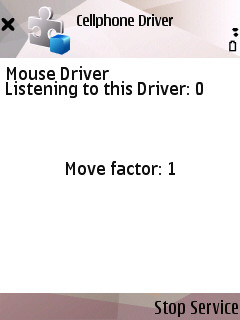
\includegraphics[width=\linewidth]{imagens/printscreen_n95}
		\caption{Printscreen do protótipo desenvolvido para Symbian.}
		\label{fig:printscreen_symbian}
	\end{minipage}
	\hfill
	\begin{minipage}[t]{0.30\linewidth}
		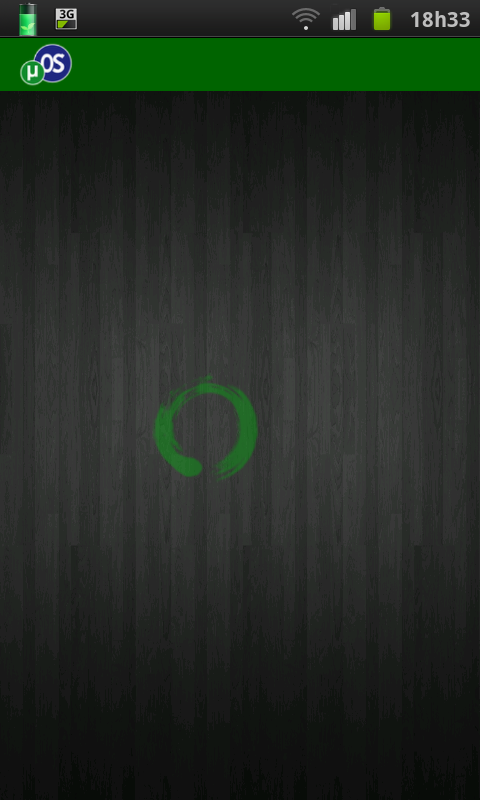
\includegraphics[width=\linewidth]{imagens/printscreen_android}
		\caption{Printscreen do protótipo desenvolvido para Android. O círculo verde representa a posição do dedo no momento da captura da imagem.}
		\label{fig:printscreen_android}
	\end{minipage}
\end{figure}
